%
\hsection{Installing PgModeler under Microsoft Windows}%
%
\begin{figure}%
\centering%
%
\subfloat[][%
We first want to download \pgls{MSYS2}. %
We therefore visit the website \url{https://repo.msys2.org/distrib}. %
We click and download \textil{msys2-x86_64-latest.exe}, if we have a 64~bit x86~system~(which usually should be the case).
\label{fig:installingPgModelerWindows01msys2Downloads}%
]{\tightbox{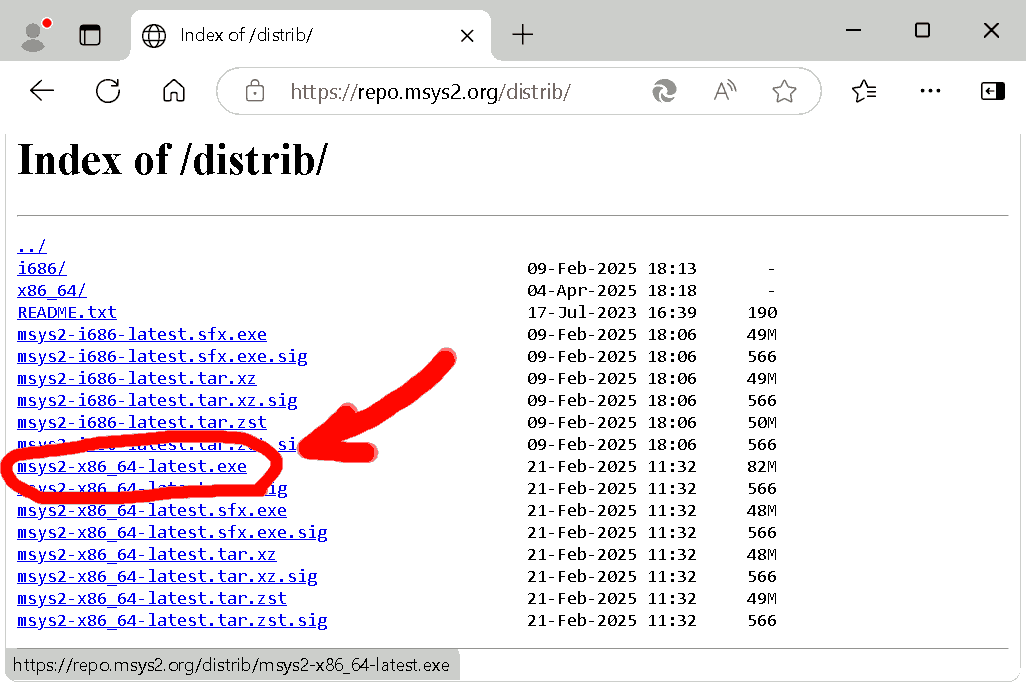
\includegraphics[width=0.7\linewidth]{\currentDir/installingPgModelerWindows01msys2Downloads}}}%
%
\floatRowSep%
%
\subfloat[][%
After the download has completed, we run the installer by clicking~\menu{Open file} or whatever option your web browser offers to run a downloaded program.%
\label{fig:installingPgModelerWindows03msys2Downloaded}%
]{\tightbox{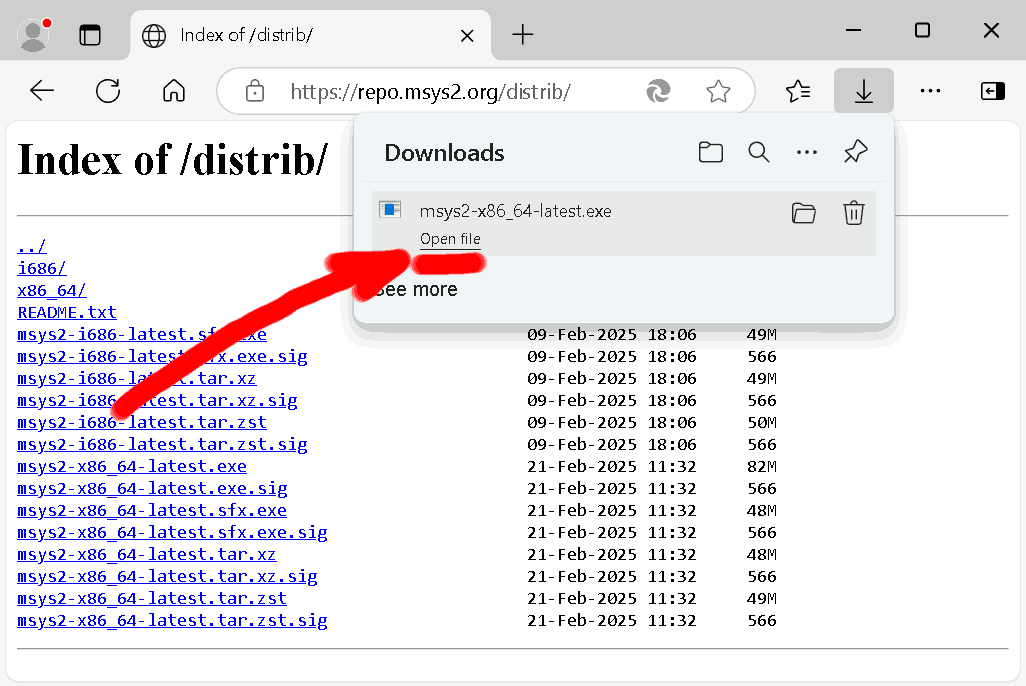
\includegraphics[width=0.7\linewidth]{\currentDir/installingPgModelerWindows03msys2Downloaded}}}%
%
\floatRowSep%
%
\subfloat[][%
We click \menu{Next} on the installer welcome screen.%
\label{fig:installingPgModelerWindows04msys2InstallerWelcome}%
]{\tightbox{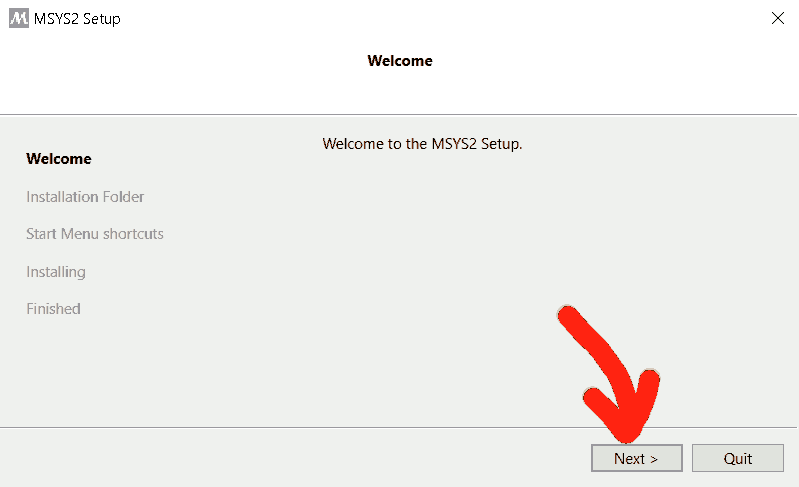
\includegraphics[width=0.7\linewidth]{\currentDir/installingPgModelerWindows04msys2InstallerWelcome}}}%
%
\caption{Installing \pgmodeler\ under \microsoftWindows\ using the \pgls{MSYS2} environment.}%
\label{fig:installingPgModeler:A}%
\end{figure}%
%
\begin{figure}%
\ContinuedFloat%
\centering%
%
\subfloat[][%
The installer wants to install \pgls{MSYS2} into \expandafter\batil{C:\\msys64}.
We agree and click \menu{Next}.%
\label{fig:installingPgModelerWindows05msys2InstallerDest}%
]{\tightbox{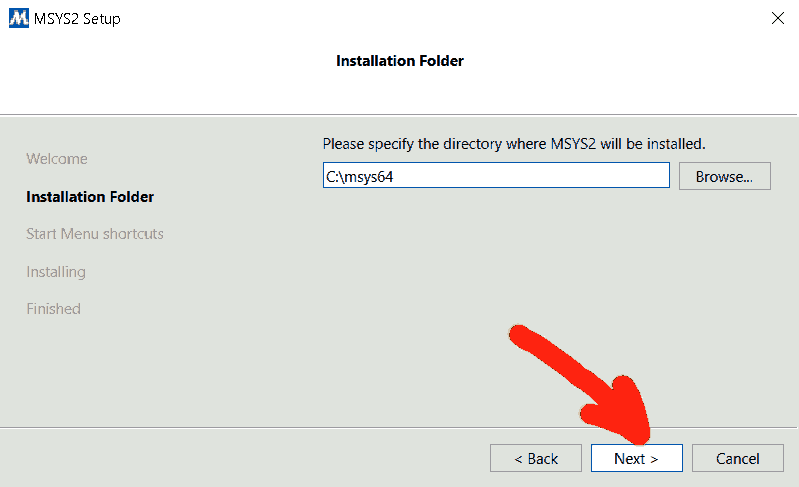
\includegraphics[width=0.7\linewidth]{\currentDir/installingPgModelerWindows05msys2InstallerDest}}}%
%
\floatRowSep%
%
\subfloat[][%
We leave the start menu settings as-is and click \menu{Next}.%
\label{fig:installingPgModelerWindows06msys2InstallerStartMenu}%
]{\tightbox{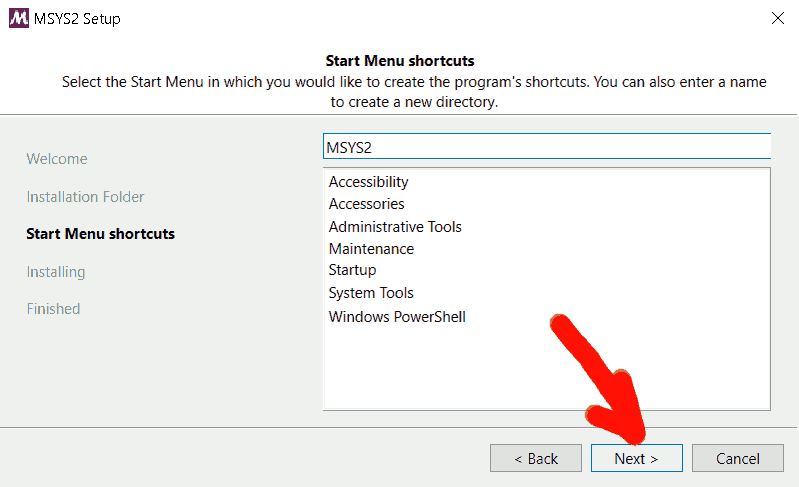
\includegraphics[width=0.7\linewidth]{\currentDir/installingPgModelerWindows06msys2InstallerStartMenu}}}%
%
\floatRowSep%
%
\subfloat[][%
The installation process begins with unpacking the archive.%
\label{fig:installingPgModelerWindows07msys2InstallerUnpacking}%
]{\tightbox{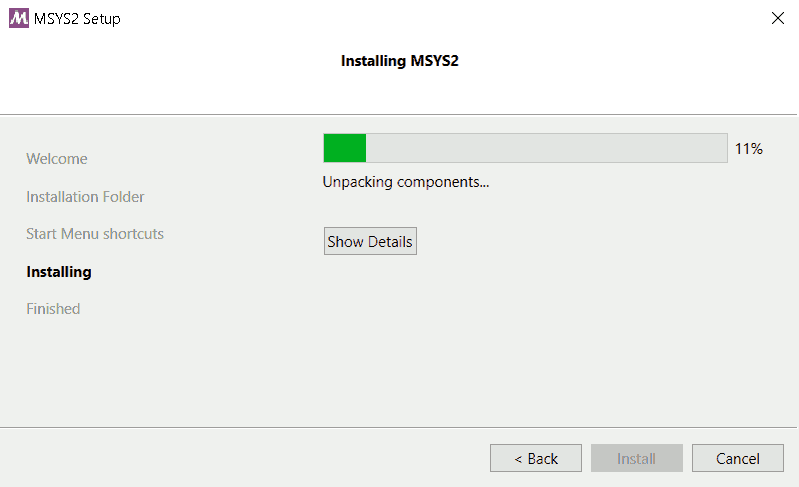
\includegraphics[width=0.7\linewidth]{\currentDir/installingPgModelerWindows07msys2InstallerUnpacking}}}%
%
\caption{Installing \pgmodeler\ under \microsoftWindows\ using the \pgls{MSYS2} environment~(continued).}%
\label{fig:installingPgModeler:B}%
\end{figure}%
%
\begin{figure}%
\ContinuedFloat%
\centering%
%
\subfloat[][%
When the installer reaches about 50\%, it can happen that it stalls for a long time. %
Just wait. It will be OK. Do not stop the process.%
\label{fig:installingPgModelerWindows08msys2InstallerWaiting}%
]{\tightbox{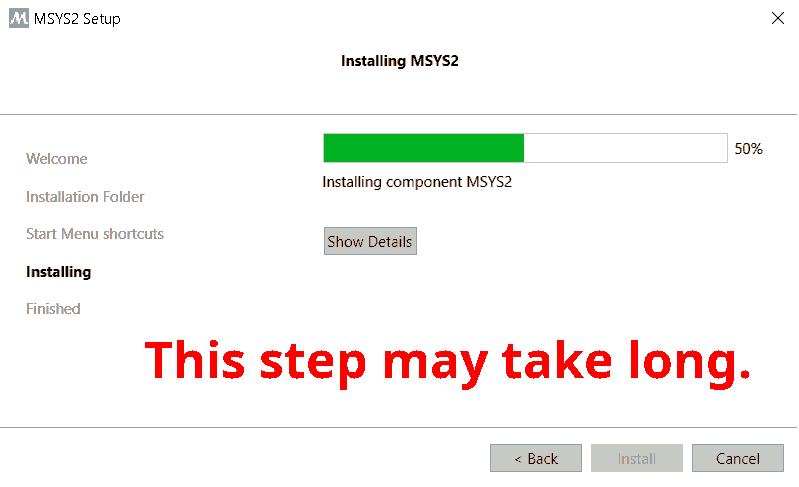
\includegraphics[width=0.7\linewidth]{\currentDir/installingPgModelerWindows08msys2InstallerWaiting}}}%
%
\floatRowSep%
%
\subfloat[][%
Eventually the installation is done. %
We can mark \inQuotes{Run \pgls{MSYS2} now.} and click on~\menu{Finish}.%
\label{fig:installingPgModelerWindows09runMsys}%
]{\tightbox{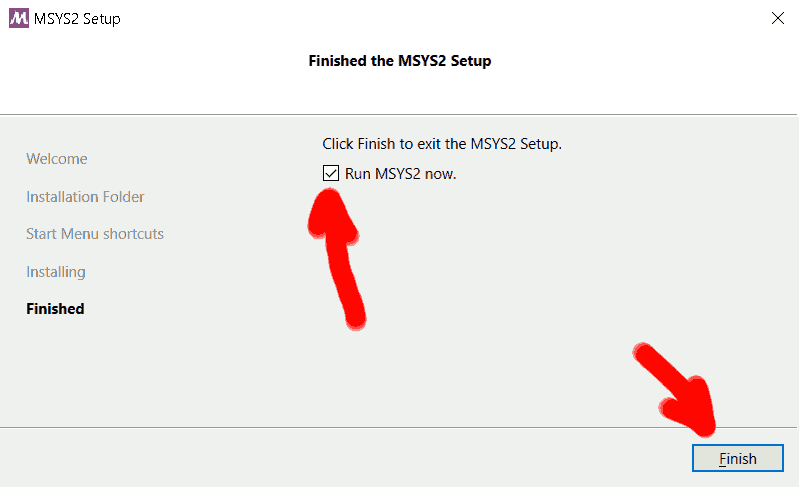
\includegraphics[width=0.7\linewidth]{\currentDir/installingPgModelerWindows09runMsys}}}%
%
\floatRowSep%
%
\subfloat[][%
From now on, we can also run \pgls{MSYS2} by entering \batil{MSYS2} in the start menu launcher and click on the \pgls{MSYS2} icon.%
\label{fig:installingPgModelerWindows10manuallyRunMsys}%
]{\tightbox{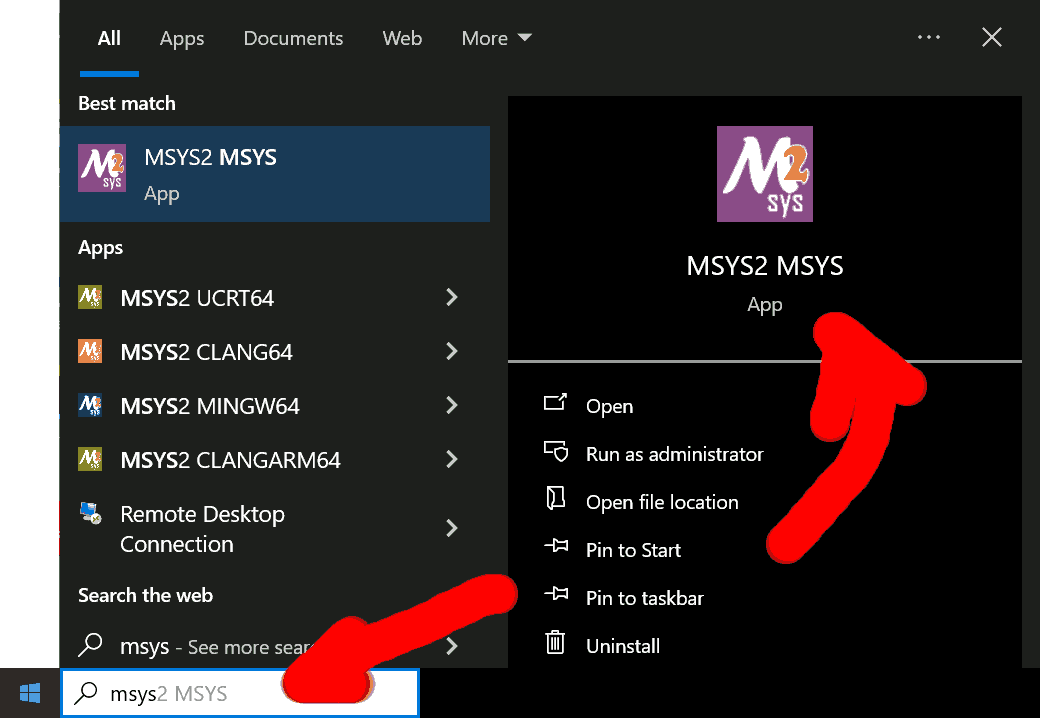
\includegraphics[width=0.7\linewidth]{\currentDir/installingPgModelerWindows10manuallyRunMsys}}}%
%
\caption{Installing \pgmodeler\ under \microsoftWindows\ using the \pgls{MSYS2} environment~(continued).}%
\label{fig:installingPgModeler:C}%
\end{figure}%
%
\begin{figure}%
\ContinuedFloat%
\centering%
%
\subfloat[][%
The \pgls{MSYS2} \pgls{terminal} is now running.%
\label{fig:installingPgModelerWindows11msysRunning}%
]{\tightbox{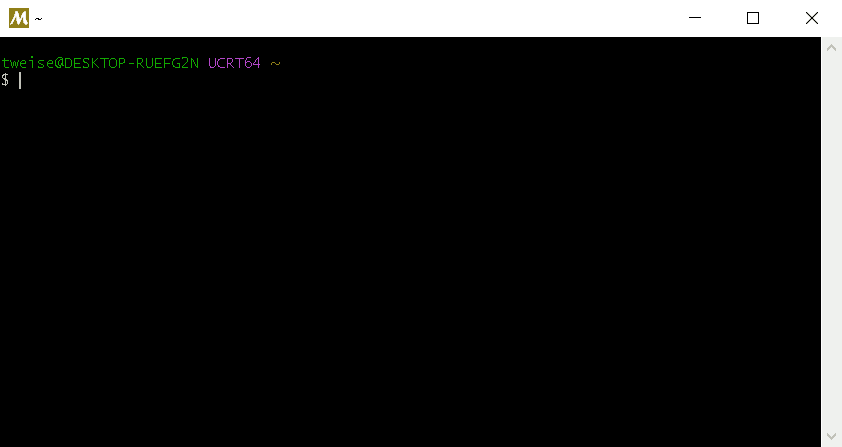
\includegraphics[width=0.7\linewidth]{\currentDir/installingPgModelerWindows11msysRunning}}}%
%
\floatRowSep%
%
\subfloat[][%
\pgls{MSYS2} uses the \bashil{pacman} package manager. %
We can search for existing \pgmodeler\ packages by typing \bashil{pacman -Ss pgmodeler} and hitting~\keys{\enter}.%
\label{fig:installingPgModelerWindows12searchPgmodelerPackages}%
]{\tightbox{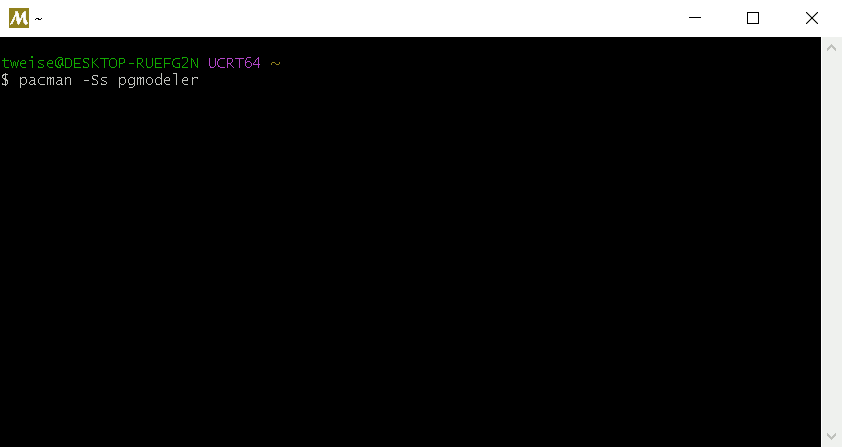
\includegraphics[width=0.7\linewidth]{\currentDir/installingPgModelerWindows12searchPgmodelerPackages}}}%
%
\floatRowSep%
%
\subfloat[][%
Indeed, we can find several! %
We want the \textil{mingw64}-one (but not the plugins). %
Next, we select the text \bashil{mingw64/mingw64-w64-x86_64-pgmodeler}.%
\label{fig:installingPgModelerWindows13pgmodelerPackages}%
]{\tightbox{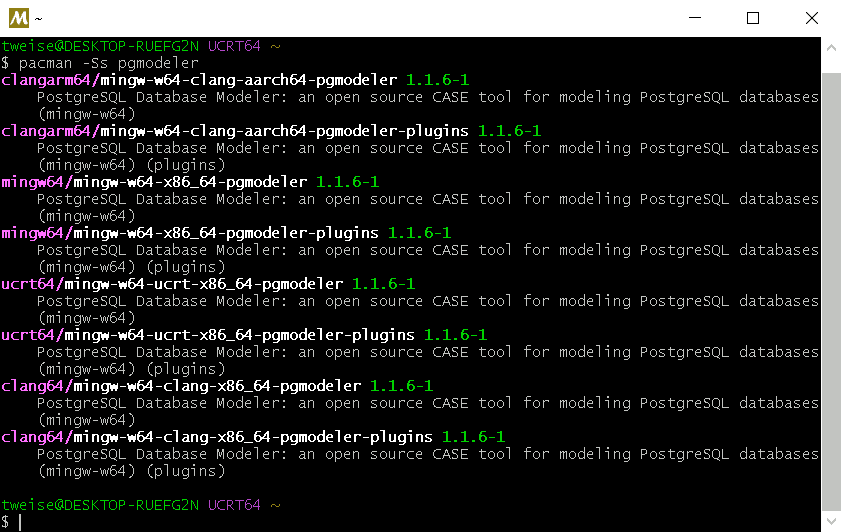
\includegraphics[width=0.7\linewidth]{\currentDir/installingPgModelerWindows13pgmodelerPackages}}}%
%
\caption{Installing \pgmodeler\ under \microsoftWindows\ using the \pgls{MSYS2} environment~(continued).}%
\label{fig:installingPgModeler:D}%
\end{figure}%
%
\begin{figure}%
\ContinuedFloat%
\centering%
%
\subfloat[][%
So we select the text \bashil{mingw64/mingw64-w64-x86_64-pgmodeler}. %
We right-click into the \pgls{terminal} and click on~\menu{Copy}.%
\label{fig:installingPgModelerWindows14copyMingwPgmodeler}%
]{\tightbox{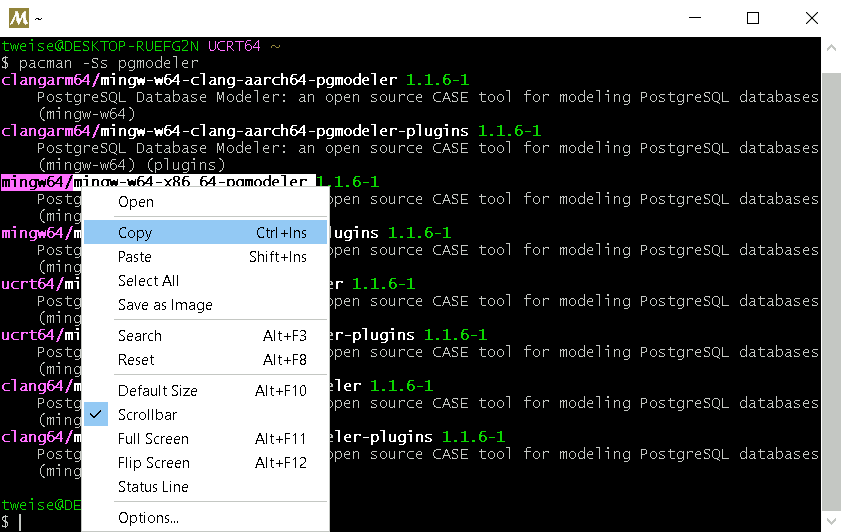
\includegraphics[width=0.7\linewidth]{\currentDir/installingPgModelerWindows14copyMingwPgmodeler}}}%
%
\floatRowSep%
%
\subfloat[][%
Then we type \bashil{pacman -S } and right-click into the \pgls{terminal} and click on~\menu{Paste}.%
\label{fig:installingPgModelerWindows15pasteMingwPgmodeler}%
]{\tightbox{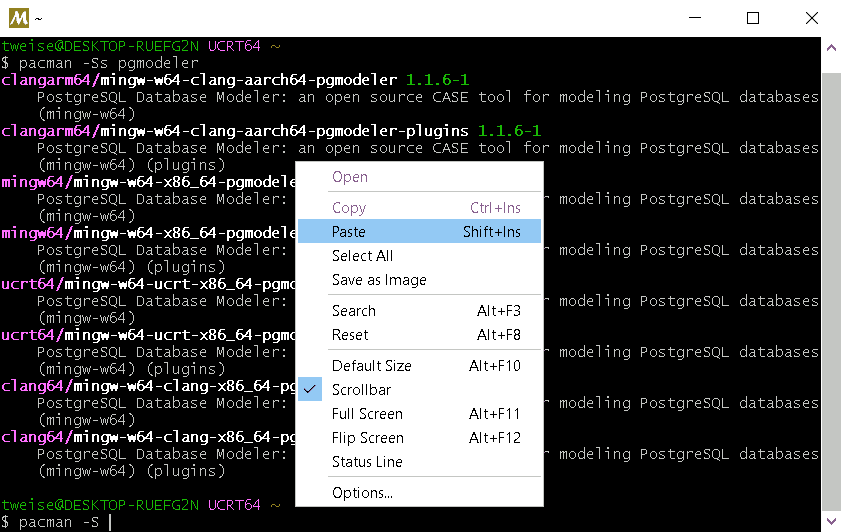
\includegraphics[width=0.7\linewidth]{\currentDir/installingPgModelerWindows15pasteMingwPgmodeler}}}%
%
\floatRowSep%
%
\subfloat[][%
This means that we wrote, in total, \bashil{pacman -S mingw64/mingw64-w64-x86_64-pgmodeler}. %
We hit~\keys{\enter}.%%
\label{fig:installingPgModelerWindows16installCommand}%
]{\tightbox{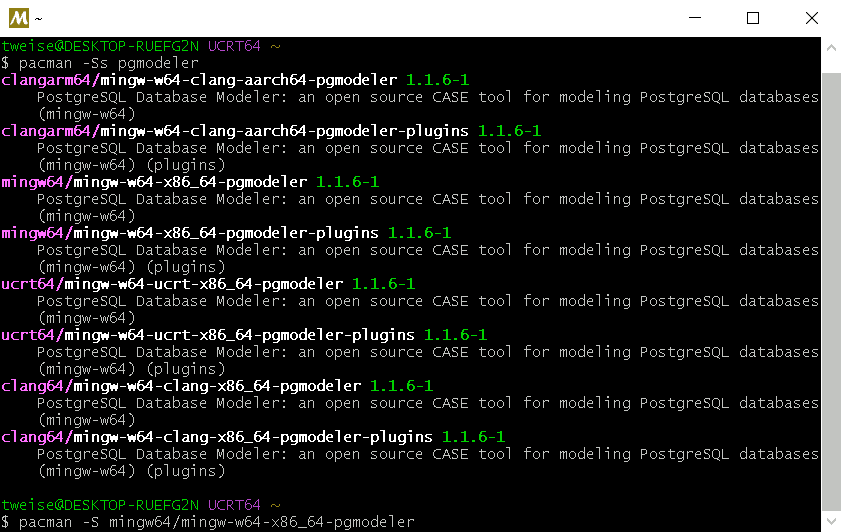
\includegraphics[width=0.7\linewidth]{\currentDir/installingPgModelerWindows16installCommand}}}%
%
\caption{Installing \pgmodeler\ under \microsoftWindows\ using the \pgls{MSYS2} environment~(continued).}%
\label{fig:installingPgModeler:E}%
\end{figure}%
%
\begin{figure}%
\ContinuedFloat%
\centering%
%
\subfloat[][%
We get a list of packages that will be installed and are asked whether we are OK with installing them. %
Devoid of emotion, we type~\keys{Y} and hit~\keys{\enter}.%
\label{fig:installingPgModelerWindows18installYes}%
]{\tightbox{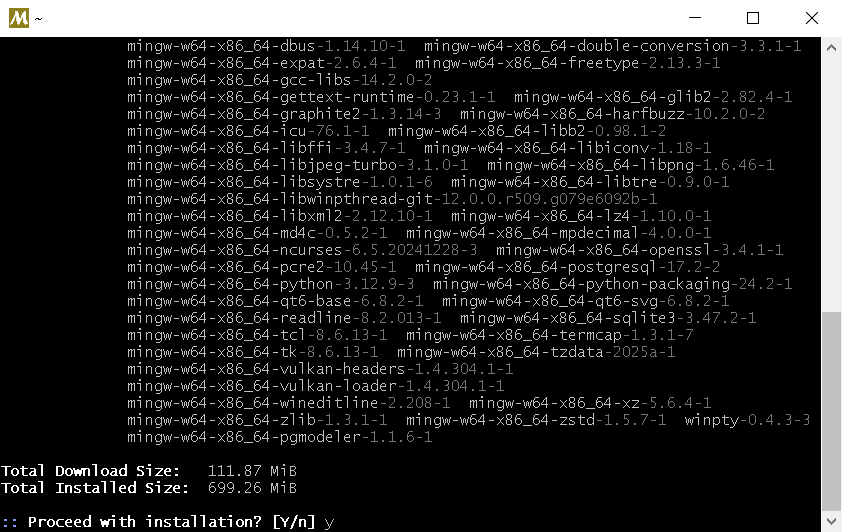
\includegraphics[width=0.7\linewidth]{\currentDir/installingPgModelerWindows18installYes}}}%
%
\floatRowSep%
%
\subfloat[][%
The packages are downloaded and installed. %
We get back to the \pgls{terminal} prompt.%
\label{fig:installingPgModelerWindows20installed}%
]{\tightbox{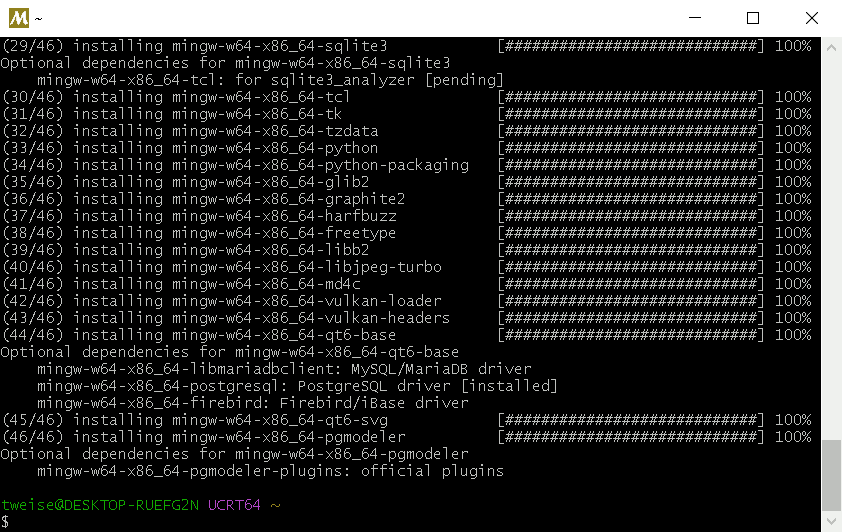
\includegraphics[width=0.7\linewidth]{\currentDir/installingPgModelerWindows20installed}}}%
%
\floatRowSep%
%
\subfloat[][%
We \textbf{close and re-open} the \pgls{MSYS2} \pgls{terminal}. %
We type \bashil{pgmodeler} in the \pgls{terminal} and hit~\keys{\enter}.%
\label{fig:installingPgModelerWindows22pgmodelerLogo}%
]{\tightbox{
\includegraphics[width=0.7\linewidth]{\currentDir/installingPgModelerWindows22pgmodelerLogo}}}%
%
\caption{Installing \pgmodeler\ under \microsoftWindows\ using the \pgls{MSYS2} environment~(continued).}%
\label{fig:installingPgModeler:F}%
\end{figure}%
%
\begin{figure}%
\ContinuedFloat%
\centering%
%
\subfloat[][%
The \pgmodeler\ main window opens! %
We could now change the theme to light, as done in \cref{fig:installingPgmodelerUbuntu09openSettings,fig:installingPgmodelerUbuntu10themeLight,fig:installingPgmodelerUbuntu11themeLightSet}.%
\label{fig:installingPgModelerWindows23pgmodelerMain}%
]{\tightbox{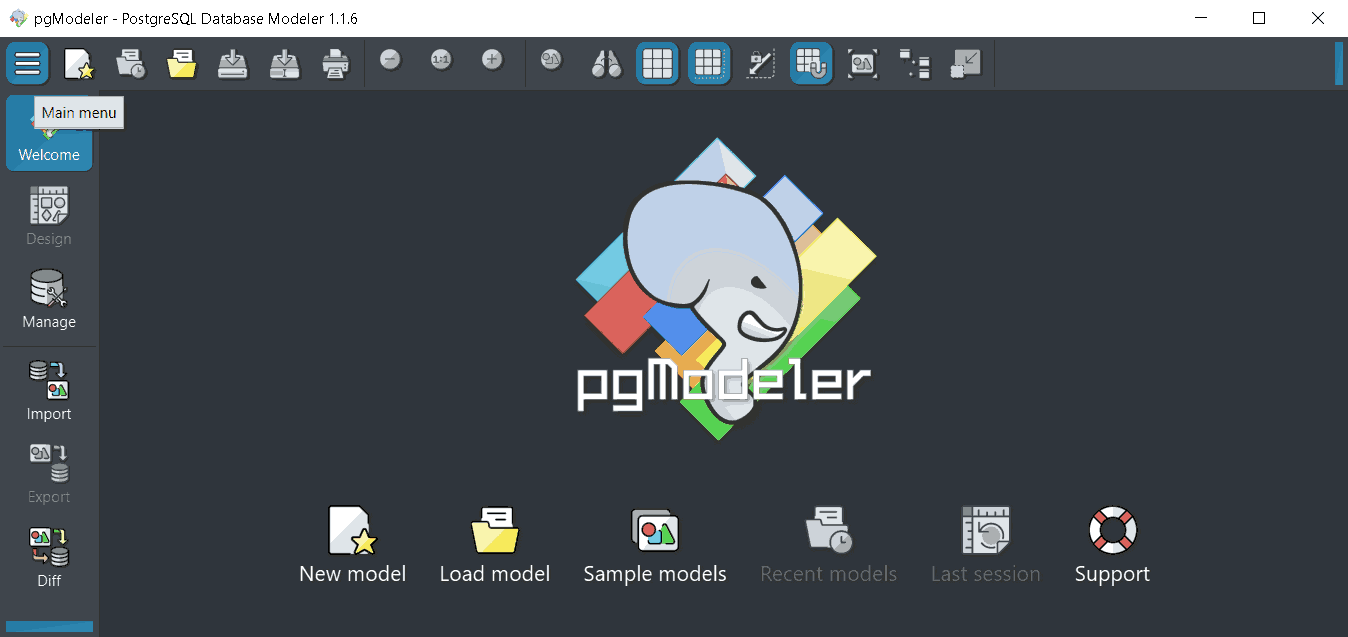
\includegraphics[width=0.7\linewidth]{\currentDir/installingPgModelerWindows23pgmodelerMain}}}%
%
\caption{Installing \pgmodeler\ under \microsoftWindows\ using the \pgls{MSYS2} environment~(continued).}%
\label{fig:installingPgModeler:G}%
\end{figure}%
%
\pgmodeler\ is a software leaning heavily to the \linux\ side.
Installing it under \microsoftWindows\ as-is is not possible~(at least not for free).
The \pgmodeler\ website recommends to first install the \glsreset{MSYS2}\gls{MSYS2} build environment under \microsoftWindows\ and then to build the program's binaries from its sources in \pgls{MSYS2}.
This is very tedious an also error-prone, as there may be issues with package incompatibilities, issues with using the right paths, etc.
Also, it requires quite some disk space.
Luckily, if we install \pgls{MSYS2}, we can also download and install \pgmodeler\ via the package manager~\bashil{pacman}~\cite{VGL2002:P,TOSID2025L:COMPMS} used by \pgls{MSYS2}.
This is much less work and we will therefore follow this path here.

Therefore, we first want to download \pgls{MSYS2}.
The download is available directly at the website~\url{https://msys2.org}, but the link provided there goes to the \github\ releases page of the project, which is not always stable.
Thus, we instead visit the website \url{https://repo.msys2.org/distrib} with out web browser.
Most \microsoftWindows\ systems are 64~bit computers of the x86~architecture.
If this is the case for your system -- which it most likely is -- then you want to download \textil{msys2-x86_64-latest.exe}.
We click on the corresponding link in \cref{fig:installingPgModelerWindows01msys2Downloads}.

The download starts.
After the it is completed, we run the installer by clicking~\menu{Open file} or whatever option your web browser offers to run a downloaded program in \cref{fig:installingPgModelerWindows03msys2Downloaded}.

The welcome screen of the installer opens in \cref{fig:installingPgModelerWindows04msys2InstallerWelcome}.
We click on \menu{Next}.
Then, we get to choose the installation location.
The installer wants to install \pgls{MSYS2} into the default location \expandafter\batil{C:\\msys64}.
We have no reason to disagree.
We leave it at this default setting and click on \menu{Next} in \cref{fig:installingPgModelerWindows05msys2InstallerDest}.
In the following screen, we can choose the start menu location.
We again have no reason to change this.
We leave the start menu settings as-is and click \menu{Next} in \cref{fig:installingPgModelerWindows06msys2InstallerStartMenu}.

The installation process begins with unpacking the archive in \cref{fig:installingPgModelerWindows07msys2InstallerUnpacking}.
In my case, when the installer reached about 50\% as shown in \cref{fig:installingPgModelerWindows08msys2InstallerWaiting}, it stalled for quite some time.
It looked like nothing happens and maybe the installer hung.
However, this was not the case:
The installation process is just doing something time consuming here.
If it seems that the installer is hanging in your system too -- simply ignore it.
Go and drink a cup of tea.
It will be OK.
Do not stop the process.

Eventually the installation is done.
In the final screen, we can mark \inQuotes{Run \pgls{MSYS2} now.} and click on~\menu{Finish}, as shown in \cref{fig:installingPgModelerWindows09runMsys}.
From now on, we can also run the \pgls{MSYS2} \pgls{terminal} manually.
We therefore enter \batil{MSYS2} in the start menu launcher of \microsoftWindows.
The icon group for \pgls{MSYS2} will appear, as shown in \cref{fig:installingPgModelerWindows10manuallyRunMsys}, and we simply click on it.

Either way, the \pgls{MSYS2} \pgls{terminal} is now running in \cref{fig:installingPgModelerWindows11msysRunning}.
As stated before, \pgls{MSYS2} uses the \bashil{pacman} package manager~\cite{VGL2002:P,TOSID2025L:COMPMS}.
We want to use this package manager to install \pgmodeler.
Therefore, we first search for existing \pgmodeler\ packages that we could install by typing \bashil{pacman -Ss pgmodeler} and hitting~\keys{\enter} as shown in \cref{fig:installingPgModelerWindows12searchPgmodelerPackages}.

Indeed, we can find several such packages.
We want the \textil{mingw64}-one, but \emph{not} the plugins package.
The suitable package in \cref{fig:installingPgModelerWindows13pgmodelerPackages} therefore is \bashil{mingw64/mingw64-w64-x86_64-pgmodeler}.
If you want to avoid typing this long name or if the name is different in your list, you simple select the text most similar to that.
Then you can right-click into the \pgls{terminal} and click on~\menu{Copy}. as shown in  \cref{fig:installingPgModelerWindows14copyMingwPgmodeler}.
Then we type \bashil{pacman -S } and right-click into the \pgls{terminal} and click on~\menu{Paste} in \cref{fig:installingPgModelerWindows15pasteMingwPgmodeler}.
This means that we wrote, in total, \bashil{pacman -S mingw64/mingw64-w64-x86_64-pgmodeler}.
This is the command to instan \pgmodeler\ under \pgls{MSYS2} in \microsoftWindows\ using \bashil{pacman}.
We hit~\keys{\enter} in \cref{fig:installingPgModelerWindows16installCommand}.

The system now shows us the package itself and the required dependencies that would be installed.
It asks us whether we are OK with downloading and installing them.
Unfazed, we type~\keys{Y} and hit~\keys{\enter} in \cref{fig:installingPgModelerWindows18installYes}.
The packages are now downloaded and installed.
We get back to the \pgls{terminal} prompt in \cref{fig:installingPgModelerWindows20installed}.

It is now important to \textbf{close and re-open} the \pgls{MSYS2} \pgls{terminal}.
After the \pgls{terminal} is opened again, we can type \bashil{pgmodeler} and hit~\keys{\enter}.
The \pgmodeler\ is starting up in \cref{fig:installingPgModelerWindows22pgmodelerLogo}.

The \pgmodeler\ main window has opened in \cref{fig:installingPgModelerWindows23pgmodelerMain}.
If you want, you can change its color theme to light, as done in \cref{fig:installingPgmodelerUbuntu09openSettings,fig:installingPgmodelerUbuntu10themeLight,fig:installingPgmodelerUbuntu11themeLightSet}.
At this stage, the program is running and usable.%
%
\FloatBarrier%
\endhsection%
%
